\documentclass[17pt, t, lualatex]{beamer}



\title{Cambio en los Ingresos de Familias Desplazadas por el Conflicto Armado}
\date{\today}
\institute[UJTL]{Universidad Jorge Tadeo Lozano}
\author{Ludwig Alvarado Becerra}

\usepackage{amsmath, amssymb, mathtools}
\usepackage[spanish]{babel}
\usepackage{biblatex}
\usepackage{hyperref}
\usepackage{xurl}

\addbibresource{referencias.bib}  % Make sure your .bib file is correctly named


\addbibresource{referencias.bib}

% Probably load as late as possible
% Other options are
% - engine=pdflatex to compile in pdfLaTeX (with different fonts),
% - mathshape=rm to use serif font for math,
% - mathsahpe=custom to not set any math font (so that you can define your own math fonts)
\usetheme[engine=lualatex, mathshape=sf, fontdir=kthpq-files/fonts/Figtree/]{kthpq}
\setmonofont{Bitstream Vera Sans Mono}[Scale=.9]

% Custom colors (see beamercolorthemecustom.sty for more details)
% \usecolortheme{custom}

% Modify the headline template: KTH-full, KTH-section-only, or KTH-frametitle-only.
% \setbeamertemplate{headline}[KTH-full]

% Custom footline
% \setfootline{left}{center}{right}

\begin{document}

\inserttitlepage

\section{Contexto}

\insertsectionpage

\begin{frame}{Contexto}

\begin{figure}[ht]
      \centering
      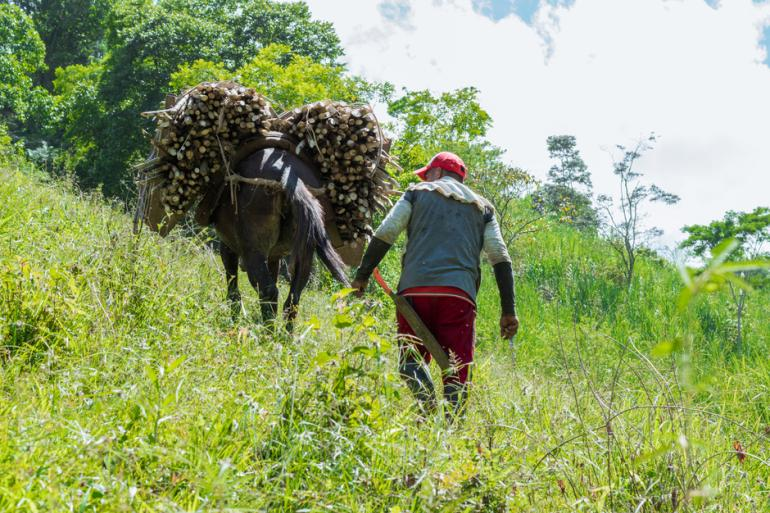
\includegraphics[width=0.5\textwidth]{img/campesino.jpg}
        \caption{Imagen obtenida de \textit{El Empleo}\cite{elempleo_campesinos_2023}}
          \label{fig:1}
\end{figure}      

\end{frame}

\begin{frame}{Contexto}

  \begin{figure}[ht]
    \centering
    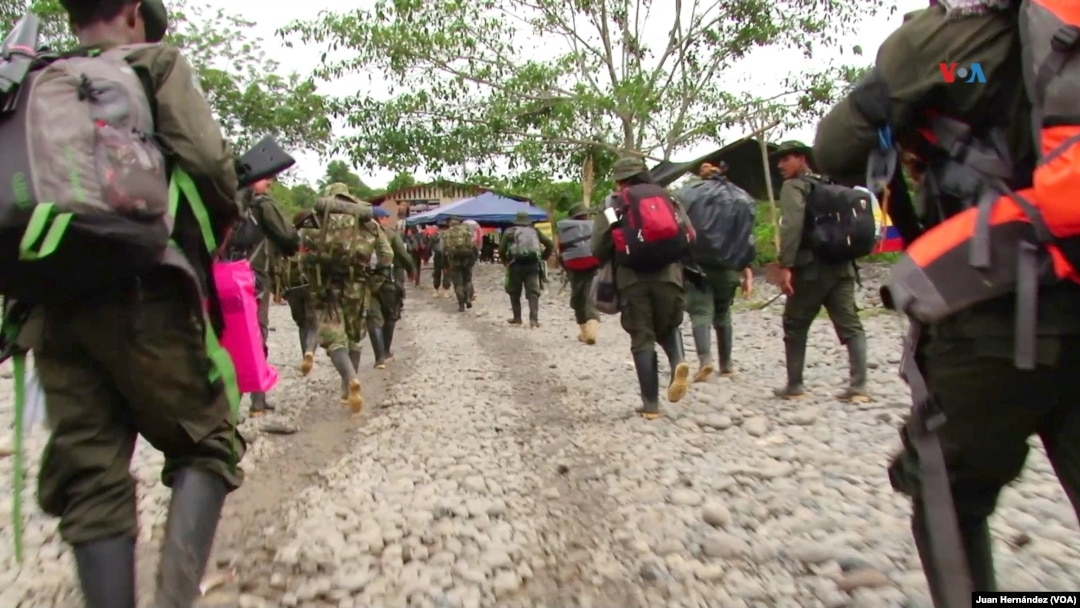
\includegraphics[width=0.6\textwidth]{img/guerrilleros.jpg}
    \caption{Imagen obtenida de \textit{Voz de América}\cite{vozdeamerica_desplazamiento_2024}}
    \label{fig:2}
  \end{figure}

\end{frame}

\begin{frame}{Contexto}

  \begin{figure}[ht]
    \centering
    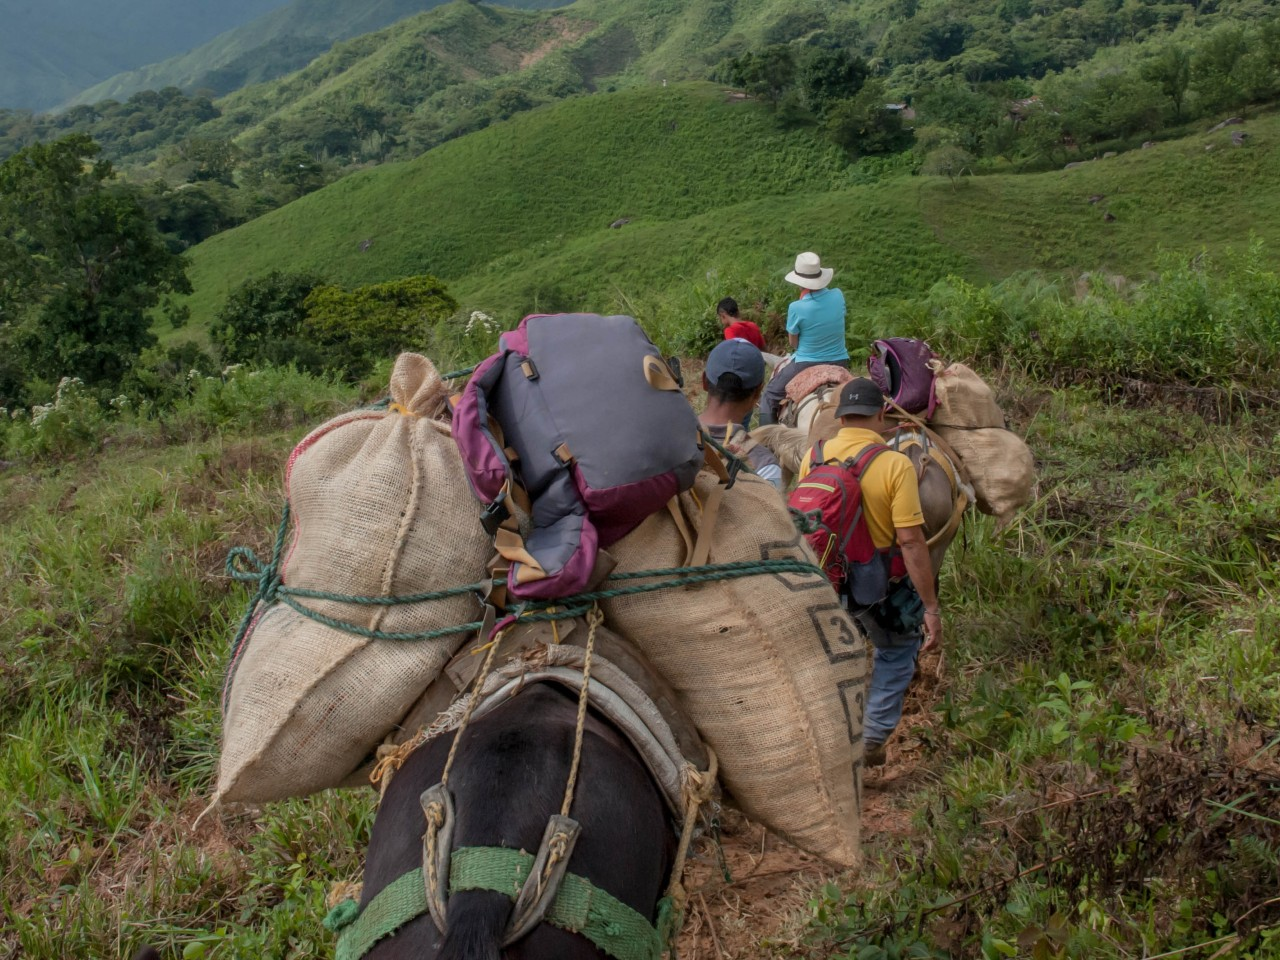
\includegraphics[width=0.45\textwidth]{img/desplazamiento.jpg}
    \caption{Imagen obtenida del \textit{Observatorio de Víctimas en Colombia}}
    \cite{unidadvictimas_observatorio_2023}
    \label{fig:3}
  \end{figure}
\end{frame}

\begin{frame}{Contexto}

  \begin{figure}[ht]
    \centering
    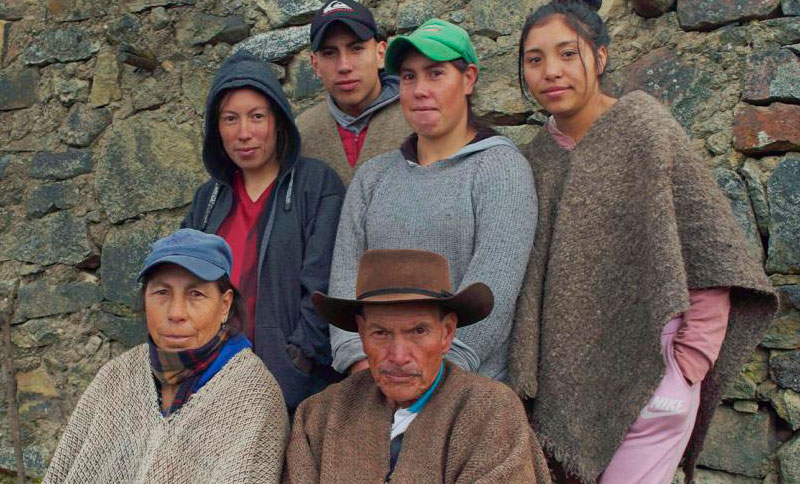
\includegraphics[width=0.45\textwidth]{img/campesinos.jpg}
    \caption{Imagen obtenida de \textit{Secretaría de cultura, recreación y deporte}}
    \cite{culturarecreacion_campesinos_2025}
    \label{fig:4}
  \end{figure}
\end{frame}

\begin{frame}{Contexto}

  \begin{columns}
    \begin{column}{0.5\textwidth}
      \begin{itemize}
        \item A cifras de hoy hay \(9.882.219\) víctimas (identificadas) por el conflicto armado.\cite{unidadvictimas_ruv_2025}
        \item El desplazamiento forzado afecta a \(8.806.334\) personas.\cite{unidadvictimas_ruv_2025}
        \item \(\sim 16.83\%\) de la población total del país.\cite{eswiki:165709323}
        \item Mayor a la población de Bogotá de 2023.\cite{eswiki:165573820}
      \end{itemize}
    \end{column}

    \begin{column}{0.5\textwidth}
      \begin{figure}[ht]
        \centering
        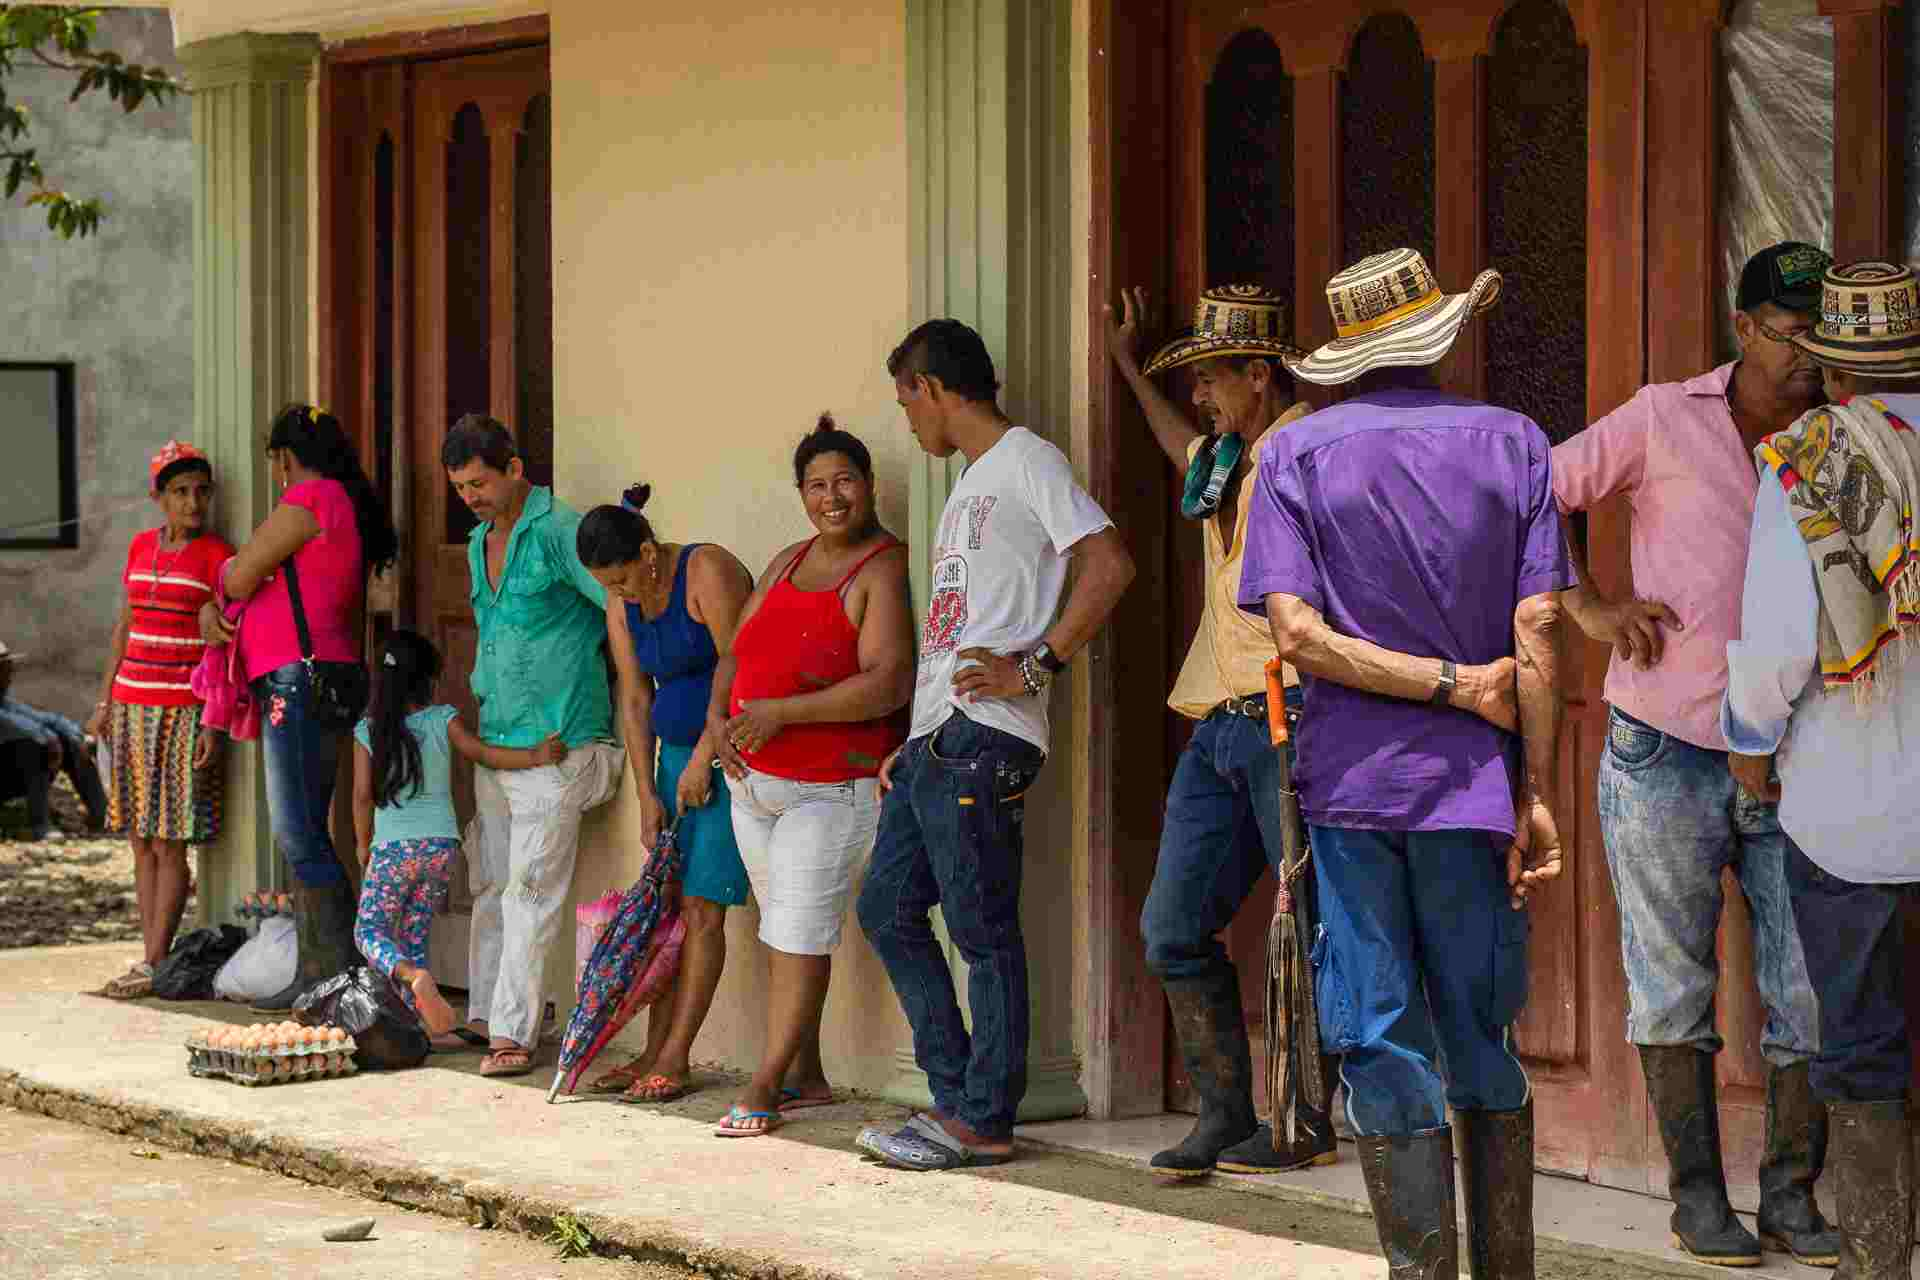
\includegraphics[width=0.8\textwidth]{img/mercado.jpg}
        \caption{Imagen obtenida de \textit{Prensa Cuestión Pública}}
        \cite{cuestionpublica_entrega_2019}
        \label{fig:5}
      \end{figure}
    \end{column}
  \end{columns}
  
\end{frame}


\section{Motivación}

\insertsectionpage

\begin{frame}{Motivación}

  \begin{columns}
    \begin{column}{0.5\textwidth}
      \begin{itemize}
        \item Conocer más acerca de los conflictos sociales del país.
        \item Modelar las interacciones entre grupos armados y la comunidad campesina.
        \item Representar cómo la economía de las familias es afectada por sufrir de estas problemáticas.
      \end{itemize}
    \end{column}

    \begin{column}{0.5\textwidth}
  \begin{figure}[ht]
    \centering
    
\includegraphics[width=0.8\textwidth]{img/motivacion.jpg}
    \caption{Ilustración perteneciente al dominio público.}
    \label{fig:6}
  \end{figure}
    \end{column}
  \end{columns}

\end{frame}

\section{Propósitos y Preguntas}

\insertsectionpage

\begin{frame}{Propósitos y Preguntas}

  \begin{columns}
    \begin{column}{0.5\textwidth}
      \begin{itemize}
        \item Identificar los factores que influyen en la migración forzada de la población campesina. 
        \item ¿Cómo se ve afectada la economía de la población desplazada en un nuevo entorno?
        \item ¿Qué relaciones existen entre las dinámicas entre grupos armados y población civil?
      \end{itemize}
    \end{column}

    \begin{column}{0.5\textwidth}
  \begin{figure}[ht]
    \centering
    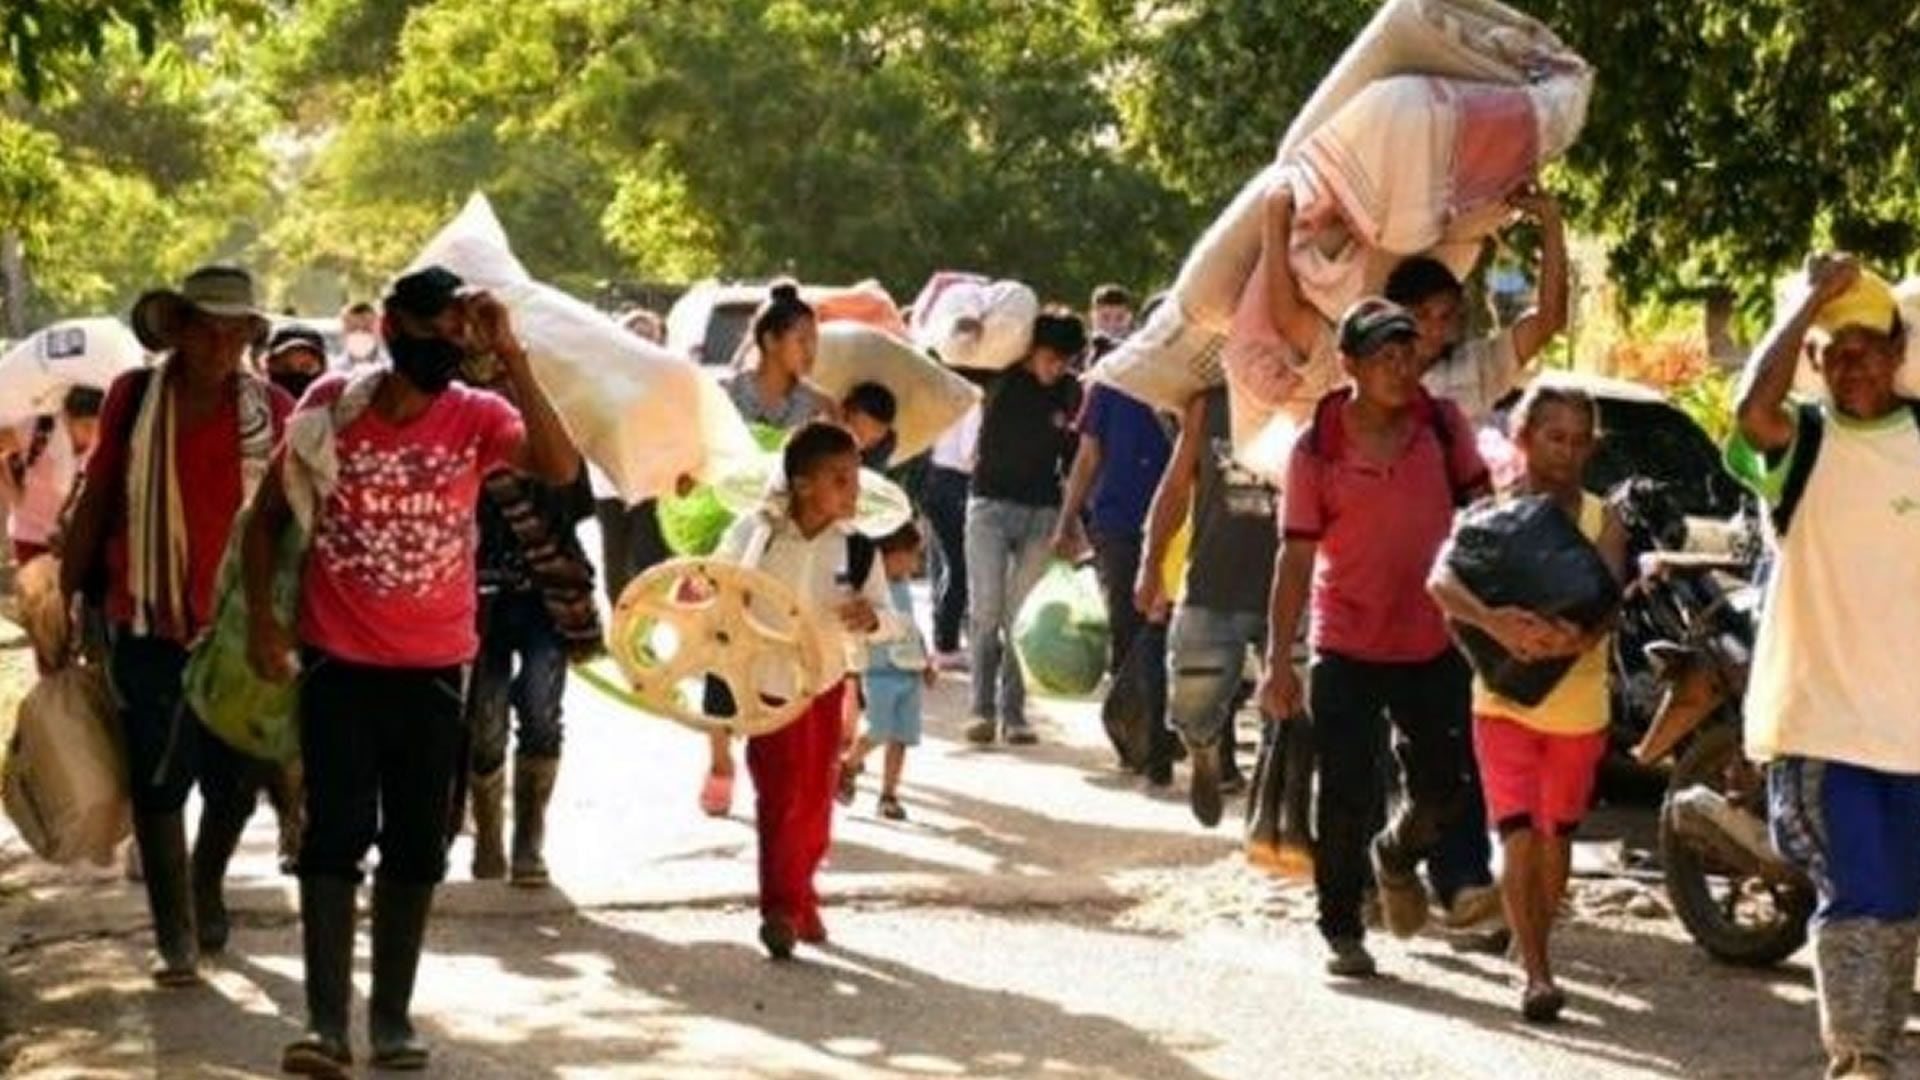
\includegraphics[width=0.8\textwidth]{img/equis.jpg}
    \caption{Imagen sacada de \textit{Infobae}\cite{infobae}}
    \label{fig:7}
  \end{figure}
    \end{column}
  \end{columns}

\end{frame}

\section{Posibles Modelos}

\insertsectionpage

\begin{frame}{Posibles Modelos}

  \begin{columns}
    \begin{column}{0.5\textwidth}
      \begin{itemize}
        \item Estudia la migración en Risaralda con tres elementos; toma de decisión de migrar, a partir de un modelo bayesiano; componente de atracción, a través de un modelo gravitacional; aplicación por agentes tomando la decisión.
        \item Utilizado para entender las dinámicas del departamento a nivel gubernamental.
      \end{itemize}
    \end{column}

    \begin{column}{0.5\textwidth}
  \begin{figure}[ht]
    \centering
    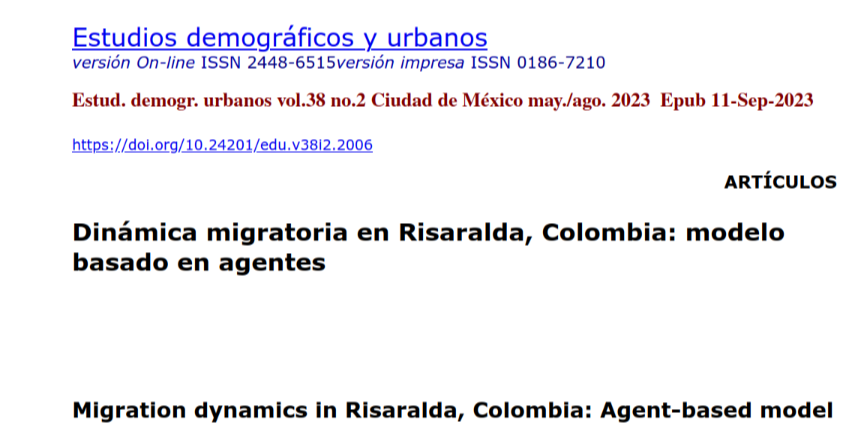
\includegraphics[width=0.8\textwidth]{img/fig2.png}
    \caption{Dinámica migratoria en Risaralda, Colombia: modelo basado en agentes\cite{renteria2023dinamica}}
    \label{fig:8}
  \end{figure}
    \end{column}
  \end{columns}

\end{frame}

\begin{frame}{Posibles Modelos}

  \begin{columns}
    \begin{column}{0.5\textwidth}
      \begin{itemize}
        \item Migración como comportamientos colectivos.
        \item Señala tres tipos de desplazamiento; normal, relativo y forzado.
        \item Da lugar a futuras investigaciones metiendo agentes de negociación como entidades con poder.
      \end{itemize}
    \end{column}

    \begin{column}{0.5\textwidth}
  \begin{figure}[ht]
    \centering
    
\includegraphics[width=0.8\textwidth]{img/fig3.png}
    \caption{Diego Felipe Gutiérrez Bedoya\cite{gutierrez2012teoria}}
    \label{fig:9}
  \end{figure}
    \end{column}
  \end{columns}

\end{frame}

\begin{frame}{Posibles Modelos}

  \begin{itemize}
    \item La mayoría de investigaciones apuntan a estudiar este problema por medio de modelos de migración.
    \item Se plantea un modelo con agentes que tengan atributos de recursos económicos y cómo estos se ven afectados al ser desplazados a un nuevo territorio.
    \item ¿Qué atributos deben tener los agentes de población campesina y grupo armado?
    \item ¿Qué supuestos se van a decidir en el mode?
    \item ¿Qué reglas va a tener el modelo?
    \item ¿Qué acciones van a tener los agentes?
  \end{itemize}

\end{frame}


\section{Referencias}

\insertsectionpage
\begin{frame}[allowframebreaks]{Referencias}
  \printbibliography
\end{frame}


\insertendpage

\end{document}
